% !TeX spellcheck = en_US
\documentclass[a4paper,fleqn,11pt]{article}

% header
%% Packages

% Styling TOC
\usepackage{tocloft}
\setlength\cftaftertoctitleskip{1cm}
\usepackage[nottoc]{tocbibind}

% Mathe Packages
\usepackage{amsmath,amssymb,epsfig,amsthm,amsfonts,bbm,textcomp}

% Grafiken
\usepackage[font=normalsize,aboveskip=0pt,belowskip=0pt,labelfont=bf]{caption}
\captionsetup{justification=justified,singlelinecheck=false}
\usepackage[edges]{forest}
\usepackage{tikz}
\usetikzlibrary{arrows,intersections,decorations.pathreplacing}
\usepackage[utf8]{inputenc}
\usepackage[T1]{fontenc}
\usepackage{lmodern}
\usepackage[english]{babel}

% Seiten Layout
\usepackage{float}
\usepackage[top=3cm,bottom=3cm,left=3cm,right=3cm,a4paper]{geometry}
\usepackage[onehalfspacing]{setspace}
\usepackage{color}
\usepackage{enumitem}
\usepackage{authblk}

% Fussnoten
\usepackage[flushmargin,hang]{footmisc}
\usepackage{listings}
\usepackage[hyphens]{url}
\usepackage[hidelinks]{hyperref}


% Tabellen
\usepackage{longtable} 			% Lange, mehrseitige Tabelle
\usepackage{tabularx}
\usepackage{array,hhline}
\usepackage{booktabs}			% Linien zwischen Zeilen
\usepackage{multirow}			% Verknüpfte Zellen über Zeilen hinweg
\usepackage{dcolumn}			% Erlaubt variable Orientierung am Decimalpunkt innerhalb einer Zelle
\usepackage{siunitx}

% Wir brauchen auch
\usepackage{todonotes}

% References
\usepackage{natbib}

% Paragraph spacing
\setlength{\parskip}{2ex}

% Spacing around headings
\usepackage[compact]{titlesec}





\begin{document}

% 1. title page
\title{\huge Forecasting Swiss Exports using Bayesian \\Forecast Reconciliation}

\author[$\dagger$]{Florian Eckert\thanks{Corresponding Author: Leonhardstrasse 21, 8092 Zürich, eckert@kof.ethz.ch, +41 44 632 29 80\\This research did not receive any specific grant from funding agencies in the public, commercial, or not-for-profit sectors.}}
\author[$\ddagger$]{Rob J. Hyndman}
\author[$\ddagger$]{Anastasios Panagiotelis}
\affil[$\dagger$]{\small KOF Swiss Economic Institute, ETH Zurich}
\affil[$\ddagger$]{\small Department of Econometrics and Business Statistics, Monash University}
\date{February 2020}

\clearpage\maketitle
\thispagestyle{empty}

\begin{abstract}
	\noindent This paper proposes a novel forecast reconciliation framework using Bayesian state space methods. It introduces an explicit identification of the coherency errors and allows for the joint reconciliation of all forecast periods. Informative priors can be used to assign weights to individual base forecasts, which makes it possible to gear high-dimensional hierarchies towards specific judgemental predictions or managerial decisions. This supports aligned decision-making at different planning horizons and at all levels of complex data structures. We conduct an extensive forecasting study on a large collection of 13,118 time series that measure Swiss merchandise exports, grouped hierarchically by export destination and product category. Overall we find strong evidence that in addition to producing coherent forecasts, reconciliation also leads to substantial improvements in forecast accuracy. The use of state space methods is particularly promising for optimal decision-making under conditions with increased model uncertainty and data volatility. \\
	
	\noindent \textbf{JEL Classification:} C32, C53, E17\\
	\noindent \textbf{Keywords}: Forecasting, Hierarchical Reconciliation, Optimal Combination, Merchandise Trade.
\end{abstract}
\clearpage
\setcounter{page}{1}

% 2. Model
\section{Introduction}\label{sec:intro}

% teaser
Forecasts are crucial inputs to the decision-making process in business analytics and macroeconomics. At an aggregate level, they are often strategic in nature and therefore subject to judgemental predictions and managerial decisions. At more disaggregate or operational levels, forecasts usually rely on statistical methods. If the data is subject to linear hierarchical constraints, predictions generated from different methods and information sets are usually not coherent. This is problematic because it may lead to contradictory conclusions and non-aligned decision-making. In addition, incoherent forecasts are often difficult to communicate. An ex post adjustment of forecasts to ensure coherence resolves these issues and has been shown to lead to substantial improvements in forecast accuracy \citep[see][and references therein]{Wickramasuriya2015}. This paper proposes a novel approach to jointly reconcile all forecasting periods using state space methods. It allows for the identification and shrinkage of coherence errors, which means specific predictions can be assigned more weight in the process of reconciliation. It may occur for instance that managerial decisions or judgmental adjustments are reflected in forecasts at the strategic level, but not in forecasts at the operational level. If the prediction at the strategic level is believed to be more accurate, the proposed method allows to reconcile all other forecasts such that they are coherent with the strategic level base forecast. This supports aligned decision-making across all operational units while maintaining a high degree of flexibility. 

% intro to reconciliation
Hierarchical data can be structured according to various characteristics, for instance geographical, organizational, societal or temporal features \citep{Kourentzes2019}. Swiss exports for example can be disaggregated geographically by destination into regions such as Western Europe, North America or Australia. These regional aggregates can then be divided further by country. Total exports can also be disaggregated into product categories such as precision instruments, textiles or vehicles and then further into subcategories such as road, rail, air and water vehicles. As such, the data has the structure of a so-called grouped hierarchy \citep[see][and references therein]{Hyndman2018}. Figure~\ref{fig:tree} gives a simple example of grouped structure with $k = 3$ levels, $m = 9$ series in total and $q = 4$ series at the most disaggregate or `bottom' level. 

\begin{figure}[H]
	\centering
	\begin{forest}
		before packing={
			forked edges,
		}
		[{$Y_0$}
		[{$Y_{A}$}
		[{$Y_{A1}$}]
		[{$Y_{A2}$}]
		]
		[{$Y_{B}$}
		[{$Y_{B1}$}]
		[{$Y_{B2}$}]
		]
		]
	\end{forest}\hspace{1cm}
	\begin{forest}
		before packing={
			forked edges,
		}
		[{$Y_0$}
		[{$Y_{1}$}
		[{$Y_{A1}$}]
		[{$Y_{B1}$}]
		]
		[{$Y_{2}$}
		[{$Y_{A2}$}]
		[{$Y_{B2}$}]
		]
		]
	\end{forest}
	\vspace{0.4cm}
	\captionab{Simple Example of a Grouped Hierarchy}{The data is structured into $k = 3$ levels, $m = 9$ time series in total and $q = 4$ time series at the bottom level.}\label{fig:tree}
\end{figure}
Since it is known that all future realizations of the data will adhere to the constraints implied by the aggregation structure, a desirable property of any forecasts is that they also respect these constraints. Such forecasts are referred to as `coherent'.  Earlier literature reduced the issue of producing coherent forecasts to one of predicting only a specific level of the hierarchy. For example, the `bottom-up' approach \citep{Gross1990} achieves coherence by producing only forecasts for the bottom level series and then summing these up according to the hierarchical structure. A major shortcoming of this approach is that disaggregate series tend to be noisy and there is a high risk of model misspecification. Features such as seasonality may be difficult to identify in the bottom level data, despite being clearly present in the aggregate series. To address this shortcoming, a `top-down' approach was proposed \citep[see][and references therein]{Athanasopoulos2009}, where the predicted top level series is disaggregated according to historical or forecasted proportions of lower levels. A compromise is given by the `middle-out' approach, where the forecasts at an intermediate level of the hierarchy are summed up to get the higher levels and disaggregated to obtain lower level predictions. A weakness of these single level methods is information loss because the time series characteristics at other levels are not taken into account.

In response to these shortcomings, there has been a tendency over the past decade towards producing forecasts for all series in the hierarchy rather than only at a single level. These are referred to as `base' forecasts and they generally do not adhere to aggregation constraints. Forecast reconciliation, introduced by \cite{Hyndman2011}, performs an ex post adjustment to base forecasts in order to produce a new set of coherent forecasts. This adjustment effectively combines predictions from all levels and in doing so `hedges' against misspecification error across the entire hierarchy. It has been shown repeatedly that linear combinations of prediction models lead to better and more robust forecasts \citep[see for instance][]{Stock2006,Conflitti2015}. There is now substantial theoretical and empirical evidence that also forecast reconciliation can significantly improve forecast accuracy for hierarchical data~\citep[see][and references therein]{Wickramasuriya2015}.

In order to encode the aggregation constraints in a hierarchy, $\textbf{y}_t$ is defined to be an $m$-vector that stacks observations at time $t$ from all series, $\textbf{b}_t$ to be a subvector of $\textbf{y}_t$ containing only the $q$ bottom level series at time $t$ and $\textbf{S}$ to be an $m\times q$ aggregation matrix. In the simple grouped hierarchy shown in Figure~\ref{fig:tree}, these are given by
\begin{align*}
\underset{(m\times 1)}{\textbf{y}_t} = \begin{bNiceMatrix}
Y_0    \\
Y_A    \\
Y_B    \\
Y_1    \\
Y_2    \\
Y_{A1} \\
Y_{A2} \\
Y_{B1} \\
Y_{B2}
\end{bNiceMatrix} \quad \underset{(m\times q)}{\textbf{S}} &=
\begin{bNiceMatrix}%[columns-width = 5mm]
1 & 1 & 1 & 1 \\
1 & 1 & 0 & 0 \\
0 & 0 & 1 & 1 \\
1 & 0 & 1 & 0 \\
0 & 1 & 0 & 1 \\
1 & 0 & 0 & 0 \\
0 & 1 & 0 & 0 \\
0 & 0 & 1 & 0 \\
0 & 0 & 0 & 1
\end{bNiceMatrix} \quad \underset{(q\times 1)}{\textbf{b}_{t}} =
\begin{bNiceMatrix}
Y_{A1} \\
Y_{A2} \\
Y_{B1} \\
Y_{B2}
\end{bNiceMatrix}.
\end{align*}
Here and in general, the matrix $\textbf{S}$ is defined such that $\textbf{y}_t = \textbf{S} \textbf{b}_{t}$ holds for all realized data. To reconcile these base forecasts, \cite{Hyndman2011} and later authors assumed the following regression structure,
\begin{align}
\textbf{y}_t(h) &= \textbf{S} \boldsymbol{\beta}_{h} + \textbf{e}_t(h),
\label{eq:regstruct}
\end{align}
where $\textbf{y}_t(h)$ is an $m$-vector containing the $h$-periods-ahead base forecasts at time $t$ for each level in the hierarchy. The error term $\textbf{e}_t(h)$ has mean zero and covariance matrix $\boldsymbol{\Sigma}_h$, and $\boldsymbol{\beta}_{h}$ represents the unknown mean of the bottom level series which combines information about forecasts at all levels. It can be estimated using the following regression equation.
\begin{align}
\label{eq:reg}
\boldsymbol{\beta}_{h} &= \left(\textbf{S}'\textbf{W}_h^{-1}\textbf{S} \right)^{-1} \textbf{S}'\textbf{W}_h^{-1}\textbf{Y}_t(h).
\end{align}
A vector of reconciled forecasts is then given by $\textbf{S} \boldsymbol{\beta}_{h}$ and will cohere to the aggregation constraints by construction. There are several potential choices for $\textbf{W}_h$. Letting $\textbf{W}_h = \textbf{I}_m$ corresponds to an ordinary least squares estimate, in the following also referred to as `no scaling'. Alternatively, a high degree of heteroskedasticity in the error terms motivates a diagonal $\textbf{W}_h$ or weighted least squares approach \citep{Hyndman2016}. Under so-called `variance scaling', weights are the variances of in-sample $h$-step ahead forecast variances, and forecasts with less accurate historical performance are down-played in reconciliation. Another alternative is the `structural scaling' approach due to \cite{Athanasopoulos2017}, whereby weights are based on the number of series aggregated at each node. More recently, the `MinT' approach was developed by \cite{Wickramasuriya2015} to allow for a $\textbf{W}_h$ that is not diagonal and exploits the covariances between the $h$-step-ahead reconciled forecast errors. The nomenclature refers to the fact that this approach minimizes the trace of the covariance matrix of reconciliation errors. These methods reconcile each forecast period independently and sometimes use a scaled version of $\textbf{W}_1$ for each $h$ to simplify computations.

% contribution
This paper contributes to the literature on forecast reconciliation in various ways. First, it introduces an explicit identification of the reconciliation errors and their representation in a state space form. This allows for the joint reconciliation of all forecasting horizons with no restrictions on the bottom level forecasts. We establish an efficient Bayesian estimation algorithm that allows for the inclusion of prior information. Second, the weights used in the reconciliation are derived from the predictive distribution rather than past variation of the base forecast errors. Our innovation is therefore particularly promising for forecasting models that allow for conditional heteroskedasticity. Third, we propose the use of informative priors to down-weight the influence of particular series irrespective of past forecasting performance. This is valuable if forecasters have strong judgmental reasons for believing that a particular model will work well in the future while other base forecasts will be less reliable. It furthermore uses informative prior distributions to address some issues in the literature, namely the occurrence of negative reconciled forecasts and singular forecast error covariance matrices. Lastly, the proposed model and existing methods are evaluated using a comprehensive grouped hierarchy of Swiss merchandise trade. Apart from the comparative analysis, this application provides insights for economic policy makers and exporting firms. Merchandise forecasts often serve as inputs into projections of other quantities such as sales, inventories, currency reserves and production capacity.

% structure
The remainder of the paper is structured as follows. Section~\ref{sec:model} introduces our novel Bayesian state space reconciliation framework and an efficient estimation algorithm.  Section~\ref{sec:datadesc} introduces in detail the data on exports of Swiss goods, using modern techniques for exploring and visualizing high-dimensional time series.  Section~\ref{sec:appl} conducts an extensive forecast evaluation that compares our proposed method with existing reconciliation techniques. Section~\ref{sec:conc} concludes.






\section{Reconciliation using Bayesian State Space Methods}\label{sec:model}

This section proposes a novel approach to forecast reconciliation. We show how to explicitly identify the reconciliation errors and estimate them as latent states that evolve over the forecasting horizon. Our method involves the use of predictive distributions instead of historical forecast errors and uses prior information to address several issues in the literature. 

\subsection{Model}
An integrated reconciliation of all forecasted periods has the advantage of combining information across the entire forecasting horizon. If a base forecast in any given forecasted period is revised downwards as a result of the reconciliation, it is likely to be revised downwards as well in the next period. This dependency can be taken into account using state space methods, which could further improve forecasting accuracy. \cite{Pennings2017} pioneered their use in order to integrate the reconciliation of incoherent information across time periods. They assume the bottom level series to be the underlying states and use elaborate state equations to capture their stochastic properties. While this takes the intertemporal dependencies nicely into account, it requires the estimation of initial states and restricts the number of usable models for the base forecasts. We propose the explicit identification of state dependent reconciliation errors $\boldsymbol{\alpha}_h$, which leaves the coherent bottom level forecasts $\boldsymbol{\beta}_h$ completely free of any assumptions or restrictions:
\begin{align}
	\label{eq:main}
	E\left[\textbf{y}_{T+h}\right] & = \textbf{S} \boldsymbol{\beta}_h = E\left[\mathbf{y}_{T}(h)\right] - \boldsymbol{\alpha}_h
\end{align}
The expected $h$-step-ahead reconciled forecasts are given by $\textbf{S} \boldsymbol{\beta}_h$.  The $m$-dimensional vector $\boldsymbol{\alpha}_h = E\left[\mathbf{y}_{T}(h)\right] - \textbf{S} \boldsymbol{\beta}_h$ contains the reconciliation biases. It can be interpreted as a fixed effect that is unique to each forecasted variable. $\textbf{S}$ is a summation matrix of order $m \times q$ and the $q$-vector $\boldsymbol{\beta}_h$ estimates the unknown mean of the reconciled bottom level forecasts. The measurement equation is then given as
\begin{align}
\label{eq:meas1}
\mathbf{y}_{T}(h) &  = \boldsymbol{\alpha}_h + \textbf{S} \boldsymbol{\beta}_h + \mathbf{e}_{T}(h), \qquad \mathbf{e}_{T}(h) \sim \mathcal{N}(\textbf{0}, \boldsymbol{\Sigma}_h).
\end{align}
The $m$-vector $\mathbf{e}_{T}(h)$ consists of $h$-step ahead base forecast errors that follow a normal distribution with mean zero and covariance matrix $\boldsymbol{\Sigma}_h$. It can be estimated by taking a sample of $n$ prediction errors $\mathbf{\hat{e}}_{T}(h)$ from the predictive distribution of $\mathbf{y}_{T}(h) $. Sampling from the predictive distribution allows also to obtain an estimate for the mean of the incoherent base forecasts $E\left[\mathbf{y}_{T}(h)\right] = \mathbf{\hat{y}}_{T}(h)$.  These draws may originate from posterior predictive distributions resulting from Bayesian forecasting models \citep{Cesur2016}, bootstrap aggregating \citep{Bergmeir2016}, model pooling \citep{Timmermann2006,Kapetanios2015}, or sampling from a fitted model \citep{Hyndman2018}. 

In order to reconcile all forecasting horizons jointly, the coherence errors $\boldsymbol{\alpha}_h$ are modeled to be state dependent. They are assumed to follow a random walk, which is very common in the literature on time-varying parameters \citep[see for instance][and references therein]{Primiceri2005}. This implies that the best guess for a coherence error in any given forecasting period is the error in the preceding period. The state equation is therefore specified as
\begin{align}
	\label{eq:state}
	\boldsymbol{\alpha}_h & = \boldsymbol{\alpha}_{h-1} + \textbf{v}_h, \qquad \textbf{v}_h \sim \mathcal{N}(\textbf{0}, \boldsymbol{\Omega}).
\end{align}
The initial state $\boldsymbol{\alpha_0}$ is the coherence error in the last observation $\textbf{y}_{T}$, which is conveniently known to be zero. It is however necessary to impose some restrictions in order to identify the parameters, which is a result of multicollinearity in equation~\eqref{eq:main}. This is quite intuitive since there is more than one unique way to reconcile incoherent forecasts. To show this formally, the coherence errors $\boldsymbol{\alpha}_h$ can be expressed equivalently by concentrating out $\boldsymbol{\beta}_h$ using the projection matrix $\textbf{P}_h = \textbf{S}(\textbf{S}'\boldsymbol{\Sigma}_h^{-1} \textbf{S})^{-1}\textbf{S}'\boldsymbol{\Sigma}_h^{-1}$. This leads to the following identity: $(\textbf{I}_m - \textbf{P}_h)\, \boldsymbol{\alpha}_h = (\textbf{I}_m - \textbf{P}_h)\, \mathbf{\hat{y}}_{T}(h).$ It is useful to define the idempotent residual maker $\textbf{M}_h = \textbf{I}_m - \textbf{P}_h$. Since $\textbf{M}_h$ is not invertible due to the presence of multicollinearity, the identity cannot be solved for $\boldsymbol{\alpha}_h$. Our identifying assumption is that $\boldsymbol{\alpha}_h$ lies in the span of $\textbf{M}_h$, in which case $\textbf{M}\boldsymbol{\alpha}_h = \boldsymbol{\alpha}_h$. This solves the identification problem and leaves the reconciliation biases as a function of the data and the residual maker $\textbf{M}_h$. This result is also intuitive since the reconciliation biases are the residuals from a regression of the base forecasts on the aggregation matrix.\footnote{See Appendix \ref{sec:proofs} for a detailed derivation}


\subsection{Estimation}\label{sec:estim}
The latent states are sampled jointly using the efficient state smoothing and simulation algorithm proposed by \cite{Chan2009}. We get the marginal distributions by approximating the joint posterior distribution via Gibbs sampling from the conditional distributions \citep{Ando2010}. Convergence is achieved very quickly, irrespective of the starting values. We therefore take a sample of size 1000 from the joint posterior distribution after a burn-in of 100 draws. The measurement equation (\ref{eq:meas1}) is stacked over the $H$ forecasting periods in order to reconcile all reconciliation error states jointly.
\begin{align}
	\label{eq:meas}
	\textbf{Y} & = \textbf{X} \boldsymbol{\alpha} + \textbf{Z} \boldsymbol{\beta} + \textbf{E}, \quad \textbf{E} \sim \mathcal{N}(\textbf{0}, \boldsymbol{\Sigma}),
\end{align}
where the parameters of interest are given by 
\begin{align*}
		\underset{((H+1)m \times 1)}{\boldsymbol{\alpha}} &= \begin{bNiceMatrix}
		\boldsymbol{\alpha}_0\\
		\vdots\\
		\boldsymbol{\alpha}_H\\
	\end{bNiceMatrix}, \quad\underset{(Hq \times 1)}{\boldsymbol{\beta}} = \begin{bNiceMatrix}
	\boldsymbol{\beta}_1\\
	\vdots\\
	\boldsymbol{\beta}_H\\
\end{bNiceMatrix}, \quad \underset{(Hm\times Hm)}{\boldsymbol{\Sigma}} = \begin{bNiceMatrix}
\boldsymbol{\Sigma}_1 & & \\
& \ddots & \\
& & \boldsymbol{\Sigma}_H \\
\end{bNiceMatrix}.
\end{align*}
The unreconciled base forecast means $\mathbf{\hat{y}}_{T}(h)$, the summation matrices and some further identities are stacked accordingly into
\begin{align*}
	\underset{(Hm \times 1)}{\textbf{Y}} = \begin{bmatrix}
		\mathbf{\hat{y}}_{T}(1) \\
		\vdots\\
		\mathbf{\hat{y}}_{T}(H) \\
	\end{bmatrix}, \quad \underset{(Hm \times (H+1)m)}{\textbf{X}} = \begin{bNiceMatrix}
		  & \textbf{I}_m & & \\
		\textbf{0} & & \ddots &\\
		  & & & \textbf{I}_m \\
	\end{bNiceMatrix},  \quad \underset{(Hm \times Hq)}{\textbf{Z}} = \begin{bNiceMatrix}
	\, \textbf{S} & & \\
	& \ddots &\\
	& & \textbf{S} \, \,\\
\end{bNiceMatrix}.
\end{align*}
The state equation (\ref{eq:state}) needs to be written correspondingly as
\begin{align}
	\label{eq:stackstate}
	\textbf{F}\boldsymbol{\alpha} &= \textbf{V}, \quad \textbf{V} \sim \mathcal{N}(\textbf{0}, \textbf{Q})
\end{align}
where
\begin{align*}
	\underset{(Hm \times (H+1)m)}{\textbf{F}} &= \begin{bNiceMatrix}
		 \textbf{I}_m & & & \\
		 -\textbf{I}_m & \textbf{I}_m & & \\
		  & \ddots & \ddots & \\
		  & & -\textbf{I}_m & \textbf{I}_m\\
	\end{bNiceMatrix}, \quad \underset{(Hm \times 1)}{\textbf{Q}} = \begin{bNiceMatrix}
		\boldsymbol{\Omega}_0 & & & \\
		& \boldsymbol{\Omega} & & \\
		& & \ddots & \\
		& & & \boldsymbol{\Omega} \\
\end{bNiceMatrix}.
\end{align*}
The initial state $\boldsymbol{\alpha_0}$ is known to be zero since it corresponds to the coherence error in the last observation $\textbf{y}_{T}$. It is sufficient to choose $\boldsymbol{\Omega}_0$ very small in order shrink the initial state $\boldsymbol{\alpha}_0$ towards zero. Furthermore, the stacked residual maker can then be calculated as $\textbf{M} = \textbf{I}_{Hm} - \textbf{Z}(\textbf{Z}'\boldsymbol{\Sigma}^{-1} \textbf{Z})^{-1} \textbf{Z}' \boldsymbol{\Sigma}^{-1}$. The conditional posterior distribution of $\boldsymbol{\alpha}$ is multivariate normal with
\begin{align*}
	\boldsymbol{\alpha} \sim \mathcal{N}(\textbf{a}_1, \textbf{A}_1) \quad \text{where} \quad \textbf{A}_1 &= (\textbf{F}'\textbf{Q}^{-1}\textbf{F} + \textbf{X}'\textbf{X})^{-1} \\
	\textbf{a}_1 &= \textbf{A}_1 (\textbf{X}'\textbf{M}\textbf{Y})
\end{align*}
This algorithm is computationally very efficient if block-banded matrices and sparse matrix algorithms are used. Following \cite{Chan2009}, it is even faster to compute the banded Cholesky factor of $\textbf{A}_1$ and solve for $\textbf{a}_1$ by forward- and backward substitution. The bottom-level means $\boldsymbol{\beta}$ are retrieved from
\begin{align*}
	\boldsymbol{\beta} \sim \mathcal{N}(\textbf{b}_1,\textbf{B}_1) \quad \text{where} \quad \textbf{B}_1 &= \left(\textbf{Z}'\boldsymbol{\Sigma}^{-1}\textbf{Z} + \textbf{B}_0^{-1} \right)^{-1}\\
	 \textbf{b}_1 &= \textbf{B}_1 \left(\textbf{Z}'\boldsymbol{\Sigma}^{-1} (\textbf{Y} - \textbf{X}\boldsymbol{\alpha}) + \textbf{B}_0^{-1} \textbf{b}_0 \right).
\end{align*}
The priors $\textbf{b}_0$ and $\textbf{B}_0$ should be chosen to be as uninformative as possible. An inconvenient effect of most reconciliation methods is the occurrence of negative reconciled bottom level forecasts. This might be a concern since many applications such as sales or exports do not allow for negative observations. Using a truncated normal prior, this issue can be resolved in an uncomplicated fashion by simply discarding draws of $\boldsymbol{\beta}$ that contain negative entries during the sampling process.

The covariance matrix of the state equation errors $\boldsymbol{\Omega}$ is chosen to be diagonal because the reconciliation errors are assumed to be unique for each base forecast model. The diagonal elements $\omega_1, \hdots, \omega_m$ can be retrieved from an inverse-gamma distribution:
\begin{align*}
\omega_i \sim \mathcal{IG}(c_1/2,d_1/2), \quad \text{where} \quad c_1 &= c_0 + H\\
	d_1 &= d_0 + (\boldsymbol{\alpha}_{h,i} - \boldsymbol{\alpha}_{h-1,i})'(\boldsymbol{\alpha}_{h,i} - \boldsymbol{\alpha}_{h-1,i})
\end{align*}
where $\boldsymbol{\alpha}_{h,i}$ denotes the reconciliation error of series $i \in \{1, \hdots, m \}$ at forecasting period $h \in \{1, \hdots, H\}$. We choose a weakly informative proper prior distribution with $c_0 = 3$ and $d_0 = 0.01$ in order to restrict the movement of the reconciliation biases slightly. 

The covariance matrix of the base forecast errors $\boldsymbol{\Sigma}_h$ is assumed to be diagonal as well since it can be very cumbersome to estimate in large hierarchies and for longer forecasting horizons. The diagonal elements $\sigma_{1,h}, \hdots, \sigma_{m,h}$ are therefore drawn from an inverse-gamma distribution according to
\begin{align*}
	\sigma_{i,h} \sim \mathcal{IG}(k_1/2,l_1/2), \quad \text{where} \quad k_1 &= k_0 + n\\
	l_1 &= l_0 + \mathbf{\hat{e}}_{i,T}(h)'\mathbf{\hat{e}}_{i,T}(h)
\end{align*}
The n-dimensional vector $\mathbf{\hat{e}}_{i,T}(h)$ represents the ex-ante known prediction errors for variable $i \in \{1, \hdots, m\}$, which have been obtained from the predictive distribution of the base forecasts. While this parsimonious approach has advantages when it comes to computational speed and more accurate forecasts at lower levels of the hierarchy, it is possible to estimate the full covariance matrix of historical base forecast prediction errors in the spirit of \cite{Wickramasuriya2015} or by ordering the draws from the independent predictive distributions following \cite{Jeon2019}. Both approaches would then require sampling from an inverse-Wishart distribution and are likely to require additional shrinkage priors. For our parsimonious approach using an inverse-gamma distribution, we choose a weakly informative prior distribution with $k_0 = 3$ and $l_0 = 1$. This has negligible impact on the posterior
distribution, but ensures that $\boldsymbol{\Sigma}_h$ is nonsingular in the case where a base forecast has no
variation.


\subsection{Bias Shrinkage}\label{sec:weighting}
In order to align decisions with a specific base forecast, it may be of interest to selectively shrink some reconciliation biases towards zero. This is especially useful when there exists some prior knowledge that a particular base forecast contains additional information that is not reflected in other base predictions. Since the covariance matrix of the prediction errors enters the model as a weighting matrix, it can be useful to impose prior restrictions on $\boldsymbol{\Sigma}_h$. This can be achieved using a time-invariant diagonal matrix $\boldsymbol{\Lambda}$ with $m$ weights on its diagonal. For the conjugate inverse-gamma prior described in section \ref{sec:estim}, this implies a parameter choice of $k_0 = n $ and $l_0 = (\mathbf{\hat{e}}_{i,T}(h)'\mathbf{\hat{e}}_{i,T}(h)) \lambda_i$, where $\lambda_i$ is the weight of the $i$th variable according to the corresponding entry in $\boldsymbol{\Lambda}$.
This can be interpreted as an empirical Bayes prior because it is defined using the known base forecast errors. In order to shrink the reconciliation bias towards zero, the corresponding weight $\boldsymbol{\Lambda}$ has to be less than one. At the same time, it is necessary to increase the remaining elements above one such that they are able to account for the higher reconciliation biases at their level of the hierarchy. This is achieved by constructing the weights such that the product of the diagonal elements of $\boldsymbol{\Lambda}$ remains constant at unity. As a result, the determinant and therefore the generalized variance of $\boldsymbol{\Lambda} \boldsymbol{\Sigma}_h \boldsymbol{\Lambda}'$ remains the same for each $\boldsymbol{\Lambda}$ \citep{Mustonen1997}.

Figure~\ref{fig:weights} demonstrates the impact of different prior assumptions on the estimated reconciliation biases. It features identical unreconciled forecasts of a simple hierarchy with $m=3$ series, where $Y_A + Y_B = Y_0$. For each series a sample is drawn from the predictive forecasts density, assumed to be $\mathcal{N}(4,2)$ for $Y_A$, $\mathcal{N}(6,1)$ for $Y_B$, and $\mathcal{N}(16,3)$ for $Y_0$. The horizontal axis shows draws from the unreconciled base forecasts, which are clearly incoherent. The vertical axis on the other hand shows the means of the reconciled forecasts. The diagonal line shows values where the means of base and reconciled forecasts are equal. For boxes above this diagonal line, reconciliation adjusts forecasts upwards, for boxes below the diagonal line reconciliation adjusts forecasts downwards.
\begin{figure}[H]
	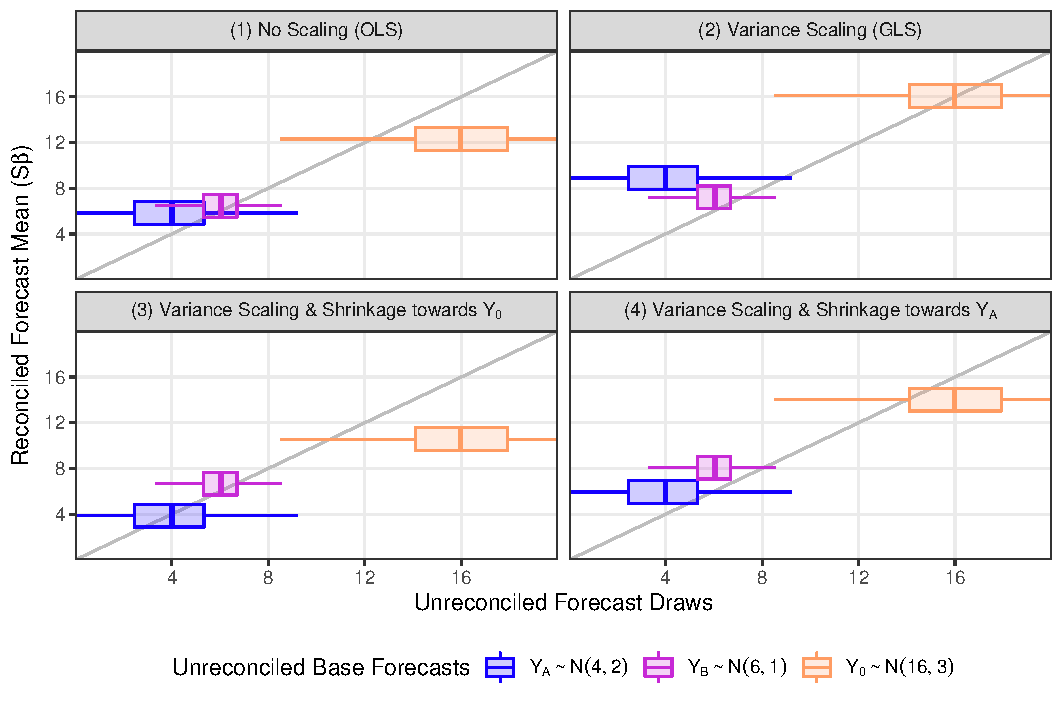
\includegraphics[width=\textwidth]{fig/fig_biases}
	\captionab{Prior Weighting Schemes}{The 45$^{\circ}$ line indicates where the unreconciled base forecasts on the x-axis are equal to reconciled forecast means on the ordinate.}\label{fig:weights}
\end{figure}
Each panel corresponds to a different prior choice for $\boldsymbol{\Sigma}_h$. Subfigure~(1) shows that the forecast biases for each margin are treated equally in an ordinary least squares regression, consequently the means of $Y_A$ and $Y_B$ are adjusted upwards while the mean of $Y_0$ is adjusted downwards. Subfigure~(2) shows reconciliation biases that are weighted with the inverse of their corresponding forecast variances. This leads to a smaller adjustment in $Y_B$ (the reconciled and base means are close) relative the others since it is more accurate. Subfigures (3) and (4) shrink the reconciled forecasts of $Y_0$ and $Y_A$ towards their base forecasts. There may exist prior information on the reliability of certain models or the requirement to fix some forecasts at specific values. This could be due to better data availability, higher suitability of a particular model or subjective judgment of the forecaster. Besides the shrinkage of specific reconciliation biases towards zero, there are several other weighting methods conceivable. Possible approaches include the weighting of each series by its level in the hierarchy or by to the number of series at each node in the hierarchy. This allows for the emulation of the `structural scaling', `bottom-up', `middle-out' and `top-down' results. A convenient feature of this is that the `middle-out' and `top-down' shrinkage work also for grouped time series, which is not the case in the standard approach.


\section{Data}\label{sec:datadesc}

We use a comprehensive dataset containing exports of Swiss goods. All time series cover a period from 1988 to 2018 in monthly frequency and are denominated in Swiss francs. They are not adjusted for seasonalities or calendar effects and data revisions are usually very insignificant. The data can be grouped by export destination and product category. The geographic hierarchy consists of 8 regions, aggregated from 245 countries and dependent territories. The categorical hierarchy follows a national nomenclature covering 12 main economic groups and 48 subgroups. This leads to a grouped hierarchy with $m = 13,118$ series containing at least one nonzero entry of which $q = 9,483$ series are at the bottom level. Figure~\ref{fig:area} shows the historical development of the regional and categorical hierarchies.\footnote{Precious metals, precious and semi-precious stones, works of art and antiques are generally omitted in business cycle research due to volatility and structural breaks. Further visualizations and a detailed statement of all categorical and geographical classifications can be found in appendix \ref{sec:data}}

As a result of its status as a small open economy in a rapidly globalizing world, Swiss exports have increased significantly since the late 1980s. Accounting for more than half of total exports, Western Europe is a key market for Swiss goods. Increasingly larger shares of exports also go to North America and East Asia with around 17\% each in 2018. Exports to Africa and the Middle East, Latin America and the Caribbean, Central Asia and Eastern Europe, South Asia, Australia and Oceania account only for about 10\% combined. The hierarchical grouping by categories is more evenly distributed, but has been subject to greater shifts in its composition. The most important categories are `Chemicals and Pharmaceuticals', `Precision Instruments' and `Machines and Electronics'. The two hierarchical groupings are quite different. The geographic hierarchy widens towards the bottom, but with a majority of the export volume going to European countries it is nevertheless highly concentrated. The categorical hierarchy on the other hand has fewer subgroups and therefore remains narrow towards the bottom. Compared to the regional hierarchy, the export volume is however more evenly distributed.

\begin{figure}[H]
	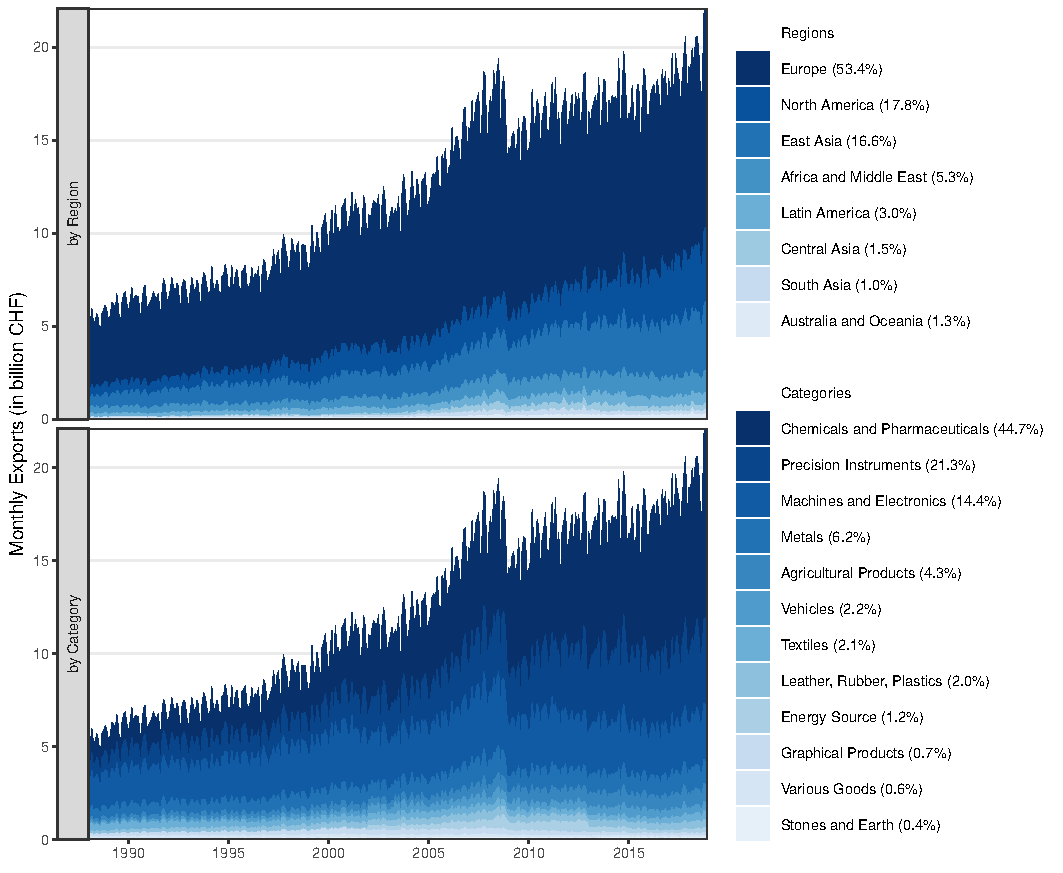
\includegraphics[width=\textwidth]{fig/fig_area}
	\captionab{Contribution to Swiss Exports of Goods}{Monthly Swiss goods exports, denominated in billion Swiss francs, not adjusted for seasonalities or calendar effects. Average export shares of the year 2018 in parentheses.}\label{fig:area}
\end{figure}


A common assumption is that series at the top level of a hierarchy are easier to forecast. Due to the aggregation involved, they are usually less noisy and exhibit more predictable characteristics such as strength of seasonality, trend, spectral entropy and serial correlation. \cite{Kang2017} measure this by extracting a number of time series features from the data that are commonly associated with better predictability. They then construct a measure of predictability for each time series by estimating principal components from these features. Figure~\ref{fig:feature} shows the first principal component, which accounts for a large share of the variation in these predictability features. It is evident that there exists a strong correlation between predictability and export volume.

\begin{figure}[H]
	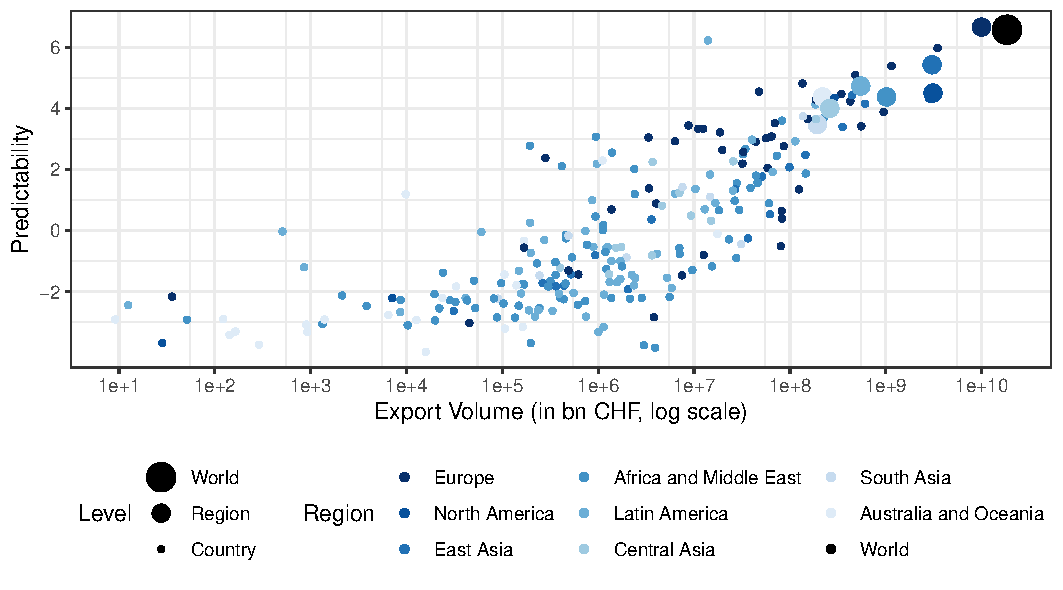
\includegraphics[width=\textwidth]{fig/fig_confetti}
	\captionab{Predictability of Different Levels in a Hierarchy}{Predictability is defined as the first principal component of a large number of time series features described in \cite{Kang2017}.}\label{fig:feature}
\end{figure}


\section{Reconciliation of Export Forecasts}\label{sec:appl}

This section provides empirical evidence for the benefits of optimal hierarchical combination. It compares the performance of different reconciliation methods and explores which data characteristics profit in particular from hierarchical combination. The setup of our comprehensive pseudo-realtime forecasting exercise is described in the following.

A large hierarchy of Swiss goods exports is used to test the Bayesian reconciliation framework and various competing methods. In each month from 1995 to 2015, forecasts for all series in the hierarchy are calculated for the next 36 months. For each of the 13,118 series, we use a few univariate benchmark models to get the base forecasts. It should be noted that these are not necessarily the best model choice since we do not take into account important covariates such as exchange rates, relative prices or global economic developments. Our focus is to show the advantages of reconciliation relative to base forecasts rather than to obtain the best possible base forecasts. We use an autoregressive integrated moving average model (ARIMA), an exponential smoothing state space model (ETS) and a seasonal random walk model (RW). As described in \cite{Hyndman2008}, the model for each series is parameterized automatically based on the Akaike Information Criterion. In order to get samples from the predictive densities, $n = 1000$ sample paths are simulated from each fitted model using Gaussian errors. With the exception of the volatile period during the Great Recession, the ARIMA and ETS approaches outperform the Random Walk on average for series at every level and forecasting horizon. All results in the following subsection will therefore rely on ARIMA forecasts.\footnote{A detailed description of the methodology and comparisons of forecasting methods, horizons and accuracy measures can be found in Appendix~\ref{sec:robust}.}

These incoherent forecasts are then reconciled using several basic single level and optimal combination methods. The single level techniques include bottom-up, top-down and middle-out methods. The latter two can only be used for non-grouped time series and are therefore tested on the regional and categorical hierarchies separately. The combination methods used are ordinary least squares (no scaling), weighted least squares with variance scaling, weighted least sqared with structural scaling, MinT and the Bayesian state space reconciliation framework (BSR). If aggregation of the prediction errors is necessary, they are weighted with their respective export share. The reconciled forecasts are then compared to the corresponding unreconciled predictions using log relative root mean squared forecast errors \citep{Hyndman2006}.


\subsection{Comparison of Reconciliation Methods}

Figure~\ref{fig:rmse_all} shows the accuracy of all forecasts, defined as the log of the root mean squared forecasting error of the base forecasts relative to the mean squared errors of the coherent forecasts from each method. Values above zero indicate therefore better forecast performance. It is worth noting that reconciliation methods and bottom-up forecasts are the only techniques that allow for coherence across all levels of a grouped hierarchy. Top-down and middle-out reconciliations are not applicable in the case of grouped time series.

\begin{figure}[H]
	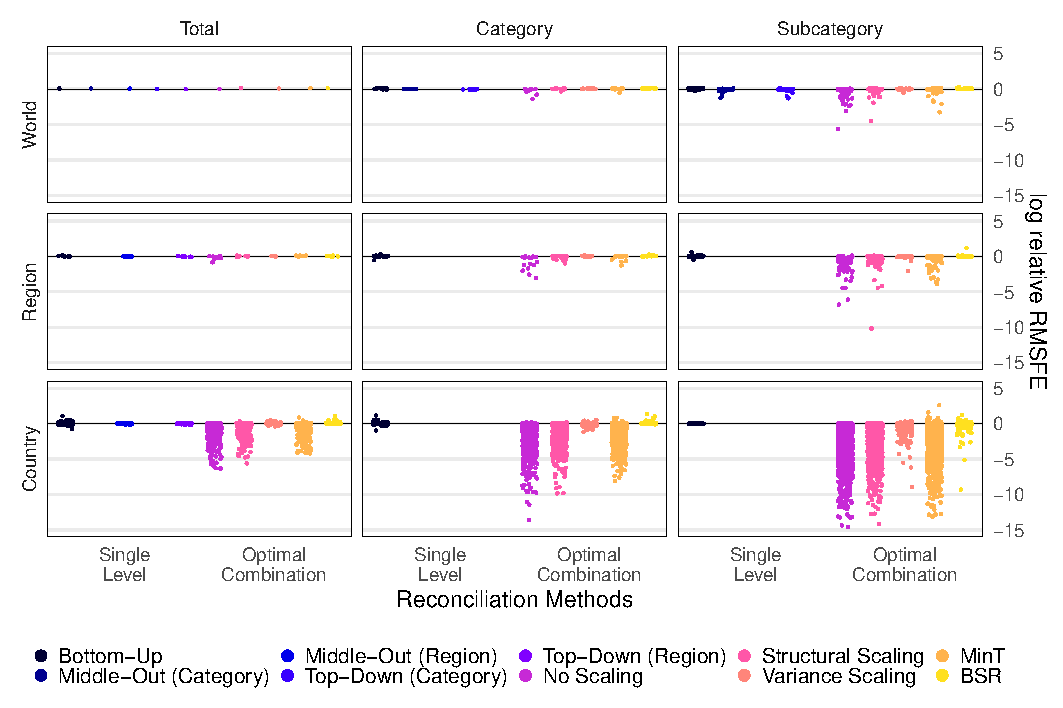
\includegraphics[width=\textwidth]{fig/fig_rmsfe_dots}
	\captionab{Relative Accuracy of Reconciliation Methods}{Values above zero indicate higher forecast accuracy relative to the unreconciled case. Forecast accuracy is given by the log of the root mean squared forecast errors of the unreconciled forecasts relative to the reconciled forecasts. Average of all forecast dates and horizons.}\label{fig:rmse_all}
\end{figure}

Figure~\ref{fig:rmse} shows that some forecasts do not benefit from reconciliation. Especially for the bottom level series, combination methods appear to decrease forecasting performance. Variance scaling and BSR are less affected by this deterioration of forecast accuracy at lower levels, probably as a result of their parsimonious parameter choice. In order to demonstrate the benefits of hierarchical combination, Figure~\ref{fig:rmse} shows average log relative RMSFEs by weighting the prediction errors at intermediate and lower levels using the corresponding share in total export volume. It is evident that single level methods do not consistently improve forecasting accuracy. The bottom-up and middle out methods fare reasonably well for the top level series, but fail to outperform the unreconciled forecasts at lower levels and are sometimes even significantly worse. Optimal combination on the other hand tends to outperform the base forecasts especially for top and intermediate level series. Especially variance scaling, MinT and BSR work well at all levels.

\begin{figure}[H]
	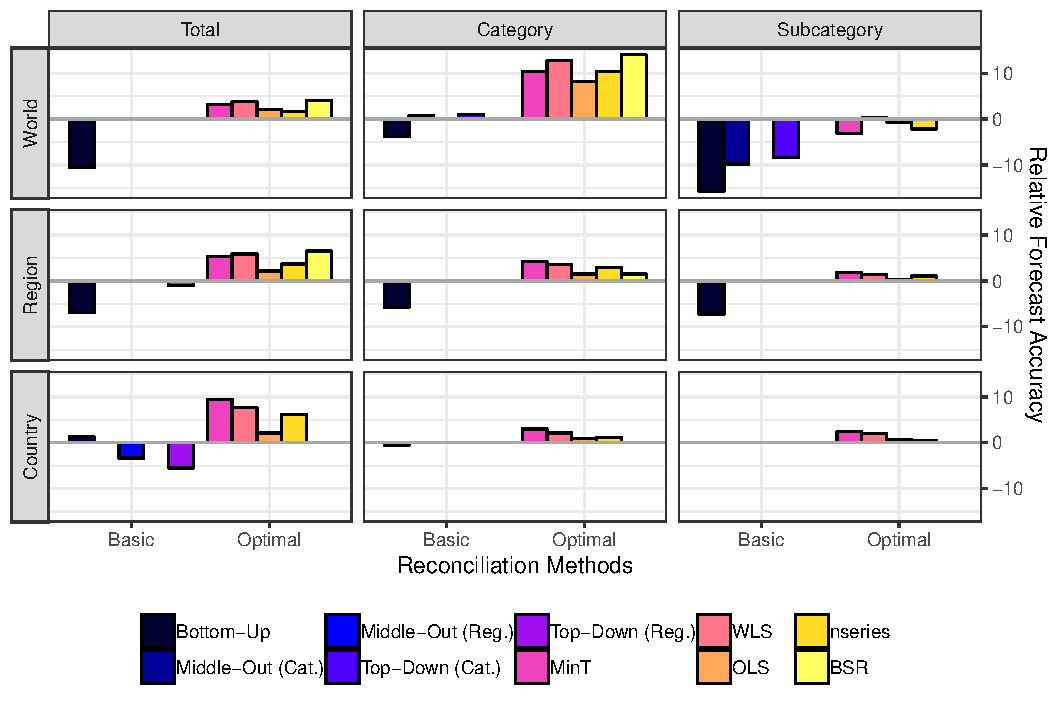
\includegraphics[width=\textwidth]{fig/fig_eval_rmse_relative}
	\captionab{Average Relative Accuracy of Reconciliation Methods}{Values above zero indicate higher forecast accuracy relative to the unreconciled case. Forecast accuracy is given by the log of the root mean squared forecast errors of the unreconciled forecasts relative to the reconciled forecasts. Errors at intermediate and bottom levels are weighted using their corresponding share in total export volume. Average of all forecast dates and horizons.}\label{fig:rmse}
\end{figure}

It is also instructive to look at the development of the relative forecasting accuracy over time in Figure~\ref{fig:rmse_time}. Even though the combination methods are more accurate on average, they do not consistently outperform the unreconciled forecasts. While the combination using no scaling does not beat the unreconciled benchmark, the remaining methods perform better and fairly similar over time. For the top level series, the benefits of reconciliation accrue mostly during times of global economic distress and corresponding appreciations of the Swiss franc. This is due to the fact that the simpler models at lower levels provide stability at times when the top level model is biased. The biggest gains can be observed during the early 2000s recession following the burst of the dot-com bubble, the global financial crisis and the following sovereign debt crisis in Europe, and the sudden appreciation of the Swiss franc after the Swiss National Bank stopped supporting the currency peg to the Euro in early 2015. Interesting is the forecasting accuracy after January 2002, when electrical energy was reclassified as a good instead of a service. The structural break in the time series leads to misspecified models, but the rigid structure imposed by the hierarchy increases forecast accuracy substantially relative to the unreconciled case.

\begin{figure}[H]
	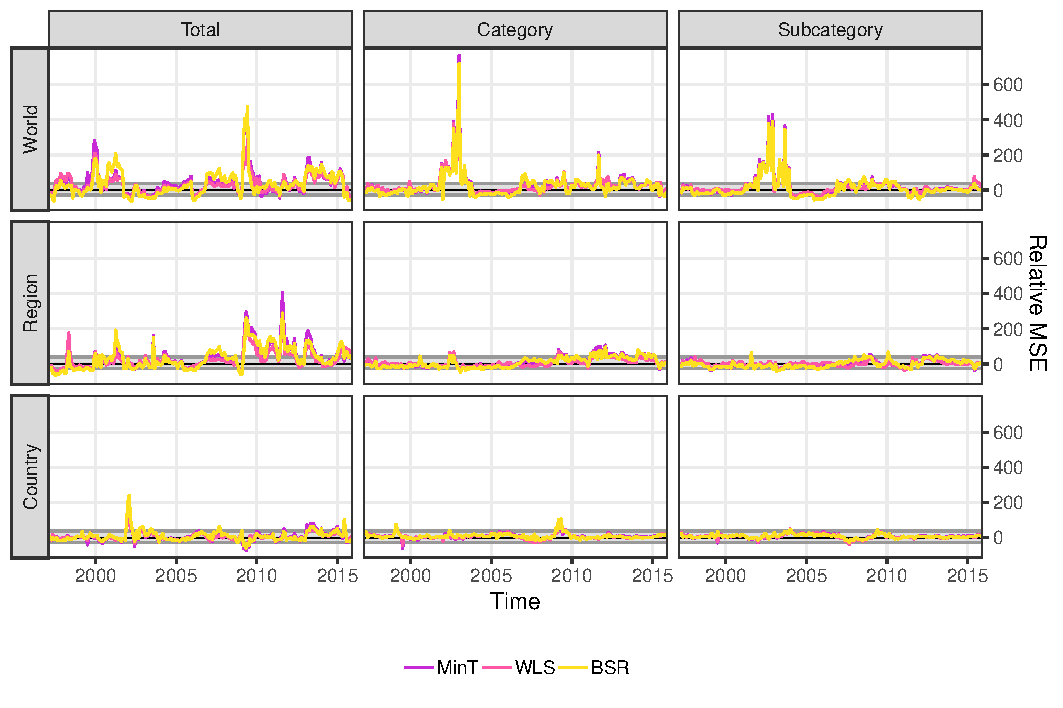
\includegraphics[width=\textwidth]{fig/fig_eval_rmse_time}
	\captionab{Relative Accuracy of Combination Methods over Time}{Values above zero indicate higher forecast accuracy relative to the unreconciled case. Forecast accuracy is given by the log of the root mean squared forecast errors of the unreconciled forecasts relative to the reconciled forecasts. Errors at intermediate and bottom levels are weighted using their corresponding share in total export volume. Average of all forecast horizons.}\label{fig:rmse_time}
\end{figure}

\subsection{Comparison of Forecasting Horizons}
In order to check whether the accuracy improvements are significant, one-sided Diebold-Mariano tests are used for the top-level series and forecasting horizons of 1, 2 and 3 years \citep{Diebold1995}. They test for significance in the difference between two squared forecast errors at various forecasting horizons, accounting for serial correlation in the squared error loss. Table~\ref{tab:dmtest} shows the p-values when testing for equality of reconciled and unreconciled forecasts, where the alternative hypothesis is that the accuracy of reconciliation methods is greater. 

\begin{table}[H]
	\caption{Diebold-Mariano Tests}\label{tab:dmtest}
	\small
	\begin{tabularx}{\textwidth}{X
		S[table-format=2.2]
		S[table-format=2.2]
		S[table-format=2.2]
		S[table-format=2.2]
		S[table-format=2.2]
		S[table-format=2.2]
		S[table-format=2.2]
		S[table-format=2.2]
		S[table-format=2.2]}
		\toprule
		 & \multicolumn{3}{c}{Entire Sample} & \multicolumn{3}{c}{Moderate Period} & \multicolumn{3}{c}{Crisis and Recovery}\\
		 & \multicolumn{3}{c}{1998 - 2018} & \multicolumn{3}{c}{1998 - 2007} & \multicolumn{3}{c}{2008 - 2018}\\
		\cmidrule(lr){2-4} \cmidrule(lr){5-7} \cmidrule(lr){8-10}
		 & \multicolumn{1}{c}{1} & \multicolumn{1}{c}{2} & \multicolumn{1}{c}{3} & 
		 \multicolumn{1}{c}{1} & \multicolumn{1}{c}{2} & \multicolumn{1}{c}{3} & 
		 \multicolumn{1}{c}{1} & \multicolumn{1}{c}{2} & \multicolumn{1}{c}{3} \\ 
		\midrule
		\multicolumn{10}{l}{\textbf{Single Level}}\\
		\addlinespace
		Bottom Up & 0.49 & 0.28 & 0.29 & 0.84 & 0.86 & 0.67 & 0.10 & 0.12 & 0.14 \\ 
		Middle Out (Category) & 0.14 & 0.05* & 0.17 & 0.28 & 0.13 & 0.09 & 0.19 & 0.16 & 0.33 \\ 
		Middle Out (Region) & 0.02* & 0.04* & 0.01* & 0.08 & 0.15 & 0.05 & 0.08 & 0.10 & 0.02* \\ 
		Top Down (Category) & 0.11 & 0.14 & 0.13 & 0.16 & 0.15 & 0.14 & 0.16 & 0.14 & 0.08 \\ 
		Top Down (Region) & 0.14 & 0.14 & 0.84 & 0.07 & 0.15 & 0.16 & 0.14 & 0.12 & 0.92 \\
		\midrule
		\multicolumn{10}{l}{\textbf{Optimal Combination}}\\
		\addlinespace
		No Scaling & 0.00** & 0.00** & 0.01* & 0.05 & 0.08 & 0.03* & 0.01* & 0.01** & 0.02* \\
		Structural Scaling & 0.05* & 0.04* & 0.09 & 0.37 & 0.40 & 0.19 & 0.00** & 0.02* & 0.06 \\ 
		Variance Scaling & 0.02* & 0.01* & 0.05* & 0.22 & 0.15 & 0.07 & 0.00** & 0.01** & 0.05* \\ 
		MinT & 0.03* & 0.01** & 0.08 & 0.14 & 0.10 & 0.13 & 0.04* & 0.03* & 0.11 \\
		BSR & 0.14 & 0.08 & 0.12 & 0.57 & 0.62 & 0.25 & 0.01** & 0.04* & 0.09 \\ 
		\bottomrule
		\addlinespace
	\end{tabularx}
	\footnotesize{Notes: Table shows p-values of one-sided Diebold Mariano tests. They are retrieved by testing differences between reconciled and unreconciled forecast errors, using the top level series and 1-year, 2-years and 3-years forecasting horizons. Significance indicated by *** p < 0.001, ** p < 0.01 and * p < 0.05.}
\end{table}
With the exception of the middle-out approaches, single level methods are not significantly more accurate than the unreconciled forecasts at all horizons. Optimal combinations are associated with lower p-values, in particular for the period of increased economic volatility after the Great Recession. Parsimonious approaches, in particular no scaling or variance scaling, appear to perform best even at longer forecasting horizons. There is however no evidence that the use of predictive distributions and state dependent reconciliation errors leads to significant gains.

\subsection{Comparison of Hierarchical Levels}
Another way to dissect the results is to identify which time series see the greatest gains in forecast accuracy from using reconciliation. Figure~\ref{fig:eval_regions} provides an overview of the relative forecast accuracy by geographic classification, using the Bayesian reconciliation framework. It is again obvious that reconciled forecasts are on average more accurate than in the unreconciled case, but not in every instance. It appears that series with a larger export volume benefit most from reconciliation. Forecasts of exports to countries in Europe, North America and East Asia are almost entirely better off than in the unreconciled case, whereas forecasts of exports to countries with a lower share, such as the islands in Oceania, tend to be worse off. In addition, time series at higher levels in a hierarchy do not necessarily profit more from reconciliation than their corresponding subcategories. The same results also hold true for the relative forecast accuracy by categories, as shown in Figure~\ref{fig:eval_categories}. Because the export shares in the categorical hierarchy are more evenly distributed, the pattern of smaller export volumes being worse off due to reconciliation is less pronounced. Results for other variance scaling methods such as weighted least squares and MinT are similar.

\begin{figure}[H]
	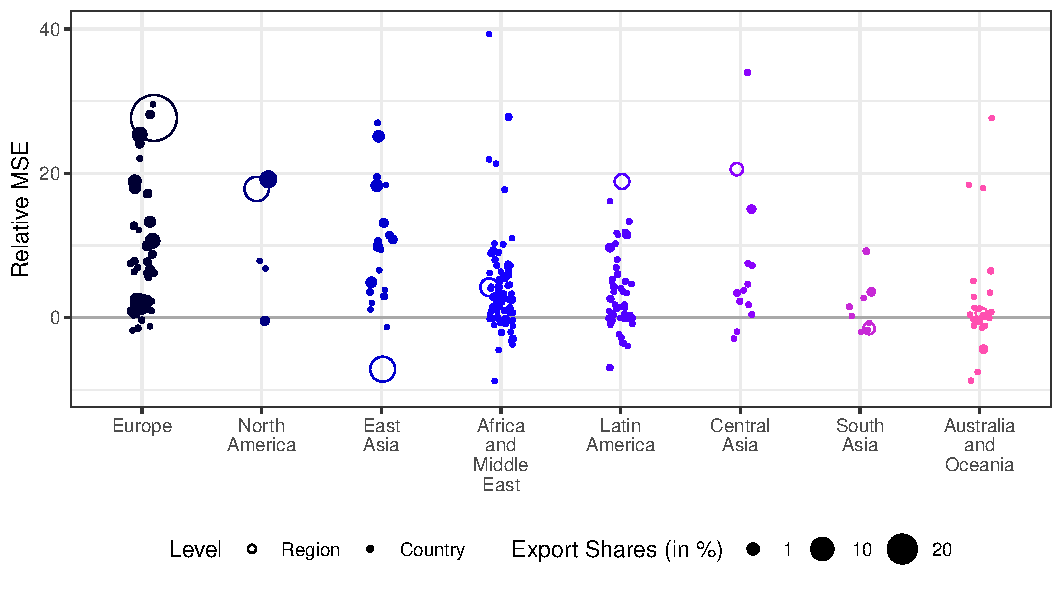
\includegraphics[width=\textwidth]{fig/fig_eval_regions}
	\captionab{Relative Accuracy of Reconciliation Methods by Regions}{Values above zero indicate higher forecast accuracy relative to the unreconciled case. Forecast accuracy is given by the log of the root mean squared forecast errors of the unreconciled forecasts relative to the reconciled forecasts. Average of all forecast dates and horizons. Reconciliation using unweighted Bayesian state space reconciliation.}\label{fig:eval_regions}
\end{figure}

\begin{figure}[H]
	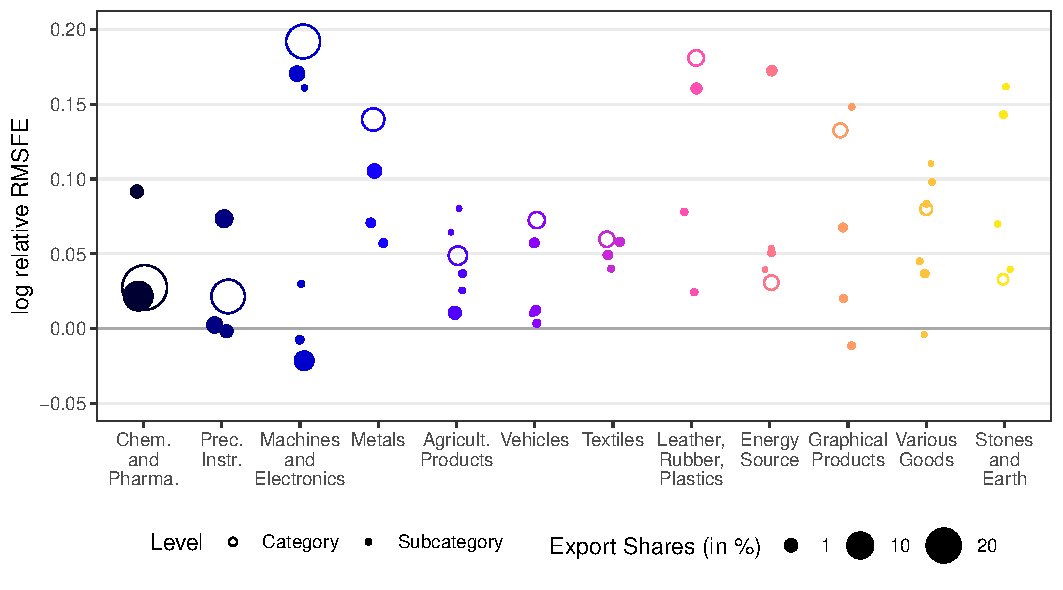
\includegraphics[width=\textwidth]{fig/fig_eval_categories}
	\captionab{Relative Accuracy of Reconciliation Methods by Categories}{Values above zero indicate higher forecast accuracy relative to the unreconciled case. Forecast accuracy is given by the log of the root mean squared forecast errors of the unreconciled forecasts relative to the reconciled forecasts. Average of all forecast dates and horizons. Reconciliation using unweighted Bayesian state space reconciliation.}\label{fig:eval_categories}
\end{figure}

%\subsection{Benefits of Weighting}\label{sec:resweight}
%
%An advantage of the general weighting scheme is that selected series can be shrunk towards their base forecast. This is particularly useful if there exists judgmental information for a specific forecast that would require adjustments for all other base forecasts in a hierarchy. An example is the reclassification of electricity as a good instead of a service. Figure~\ref{fig:fcex} shows total exports of energy sources for unweighted and weighted reconciliation.
%
%After observing the first value including electric energy in January 2002, a random walk forecast is used for this particular series. Then the series are reconciled with and without an appropriate weighting scheme. For the unweighted model on the right, the other base forecasts assume the structural break to be an outlier and dominate any information from the random walk forecast. Even though the forecaster has prior knowledge that the random walk forecast is appropriate, it is overruled in the reconciliation procedure. The only possibility is a cumbersome adjustment of the base forecasts for all other series as well.
%
%The model on the left shows the reconciliation of the same forecasts with more weight on the random walk forecast. This is done as described in Section~\ref{sec:weighting}. The diagonal entry in $\Lambda$ that corresponds to the random walk forecast is scaled down. At the same time, the remaining entries are scaled up such that the determinant of $\Lambda$ remains at 1. This forces the reconciled forecast for energy sources to stay close to its random walk base forecast. The remaining series adjust accordingly during the reconciliation procedure. As a result, the mean squared error of the forecast for energy sources in 2002 is more than 90\% lower than in the unweighted case. This also leads to significant accuracy gains at other levels; the forecast of total exports for instance is 14\% more accurate in 2002.

\section{Conclusion}\label{sec:conc}

This paper extends the literature on hierarchical forecast combination by introducing an explicit definition of the reconciliation biases and establishing a Bayesian state space framework. This allows for the joint reconciliation of all forecast periods and combines information on the coherence errors across the entire forecasting horizon. The Bayesian framework furthermore allows for the incorporation of prior information on the parameters, which enables the forecaster to introduce subjective judgment into the reconciliation. By assigning more weight to forecasts that reflect managerial predictions or judgmental adjustments, this allows for aligned decisions across operational units. In addition, informative priors avoid some issues such as the occurrence of negative reconciled forecasts and singular forecast error covariance matrices. The use of predictive densities instead of past forecast errors allows for greater flexibility in the choice of the base forecast models, taking for instance conditional heteroskedasticity into account when weighting the forecasts at different horizons. However, the approach tends to be slower than established reconciliation techniques because it requires simulation of the joint posterior distribution.

Using a comprehensive hierarchical dataset of Swiss goods exports, we demonstrate that optimal combination methods improve the forecasting accuracy significantly compared to the unreconciled case and simpler reconciliation methods. While the MinT approach shows the most improvements at higher levels, more parsimonious approaches such as variance scaling or Bayesian state space reconciliation improve the accuracy also at lower levels. The results are robust to changes in the forecasting horizon, the underlying base forecast models and the measure used to determine forecasting accuracy. Even though reconciled forecasts are significantly more accurate  on average, no reconciliation method consistently outperforms the unreconciled forecasts across the hierarchy or over time. Forecasts at aggregate levels tend to benefit more from reconciliation than the noisy series at the bottom of a hierarchy. At the same level, forecasts that account for a larger share of the total are on average more accurate after reconciliation. 

Optimal combination are shown to be particularly useful in the case of misspecified models and during periods of high volatility in the time series. In addition, state space methods lead to less outliers at lower levels, which is important for decision-making at the operational level.


% bibliography
\clearpage
\bibliography{library}
\bibliographystyle{apalike}
\clearpage

% appendix

\appendix
\section{Appendix}


\subsection{Robustness}
\label{sec:robust}

\begin{figure}[H]
	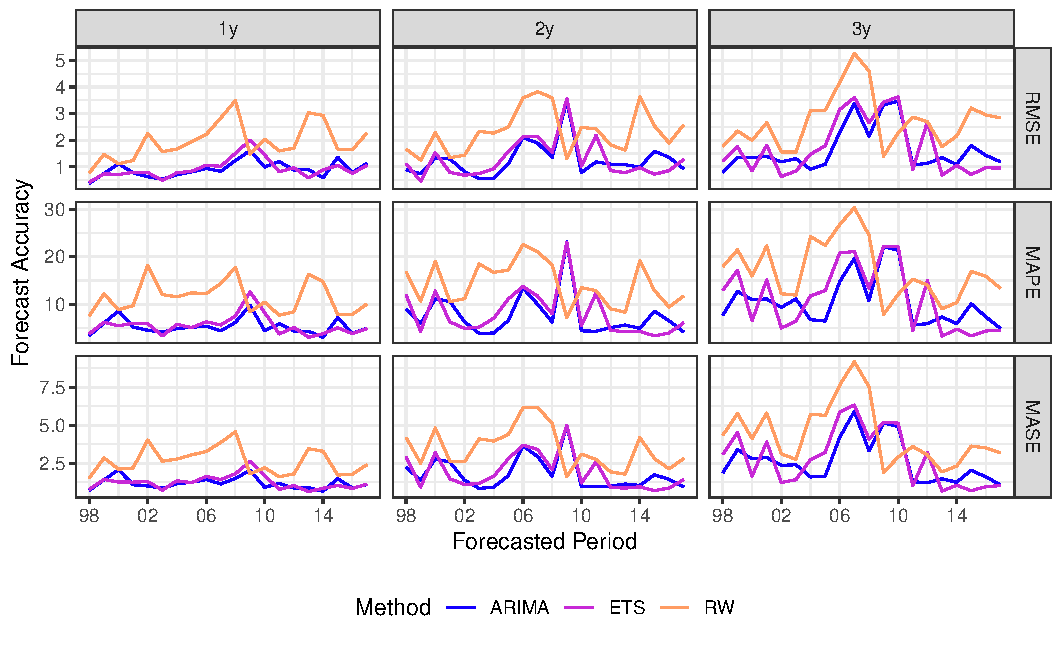
\includegraphics[width=\textwidth]{fig/fig_eval_methods_top}
	\caption{Accuracy of Forecasting Methods at the Top Level}
\end{figure}

\begin{figure}[H]
	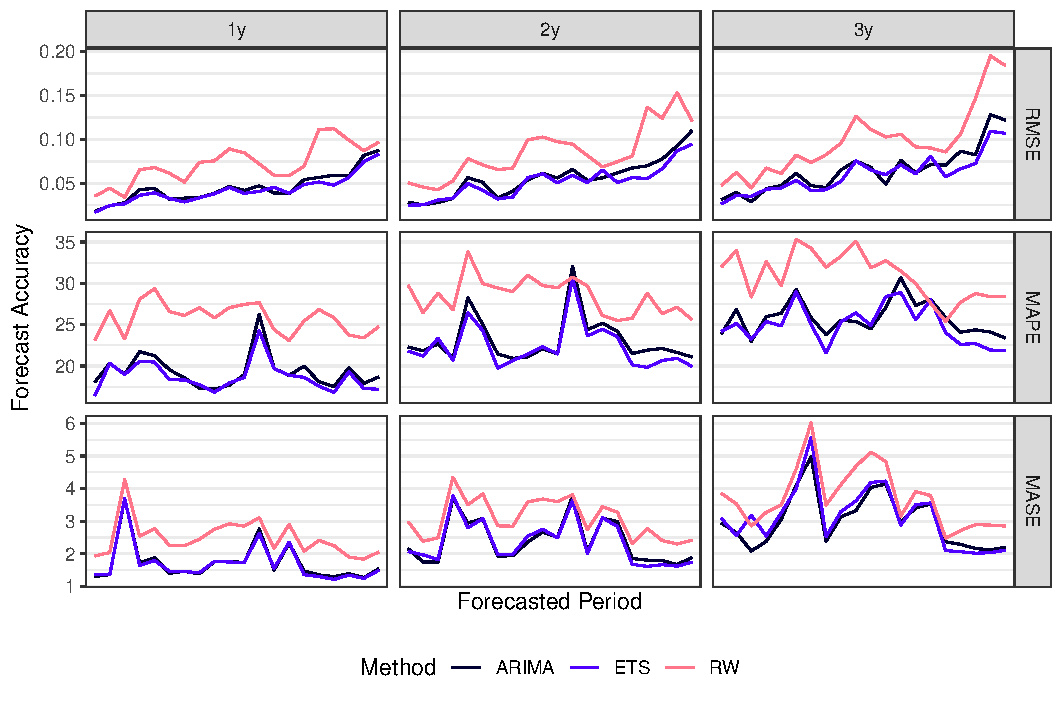
\includegraphics[width=\textwidth]{fig/fig_eval_methods_bottom}
	\caption{Accuracy of Forecasting Methods at the Bottom Level}
\end{figure}


\subsection{Data}
\label{sec:data}
The data is compiled by the Swiss Federal Customs Administration\footnote{\url{https://www.ezv.admin.ch/ezv/en/home/topics/swiss-foreign-trade-statistics.html}} and made available in a machine-friendly format on basis of a subscription.\\
% table with goods categories
\begin{small}
\begin{longtable}{p{2.5cm}p{11.5cm}}
\caption{Tariff Numbers and Descriptions of Goods}\\
\toprule
\normalsize{Tariff Number} & \normalsize{Description}\\
\midrule
\endfirsthead
\multicolumn{2}{@{}l}{\ldots continued}\\
\toprule
\normalsize{Tariff Number} & \normalsize{Description}\\  
\midrule
\endhead
\bottomrule
\multicolumn{2}{r@{}}{continued \ldots}\\
\endfoot
\bottomrule
\endlastfoot
	01	&	Forestry and agricultural products, fisheries	\\
\enskip	01.1	&	Food, beverages and tobacco	\\
\enskip	01.2	&	Feeding stuffs for animals	\\
\enskip	01.3	&	Live animals	\\
\enskip	01.4	&	Horticultural products	\\
\enskip	01.5	&	Forestry products (not firewood)	\\
\enskip	01.6	&	Products for commercial/industrial further processing such as oils, fats, starches, plants and vegetable parts, etc.	\\
\midrule
	02	&	Energy source	\\
\enskip	02.1	&	Solid combustibles	\\
\enskip	02.2	&	Petroleum and distillates	\\
\enskip	02.3	&	Gas	\\
\enskip	02.4	&	Electrical energy	\\
\midrule
	03	&	Textiles, clothing, shoes	\\
\enskip	03.1	&	Textiles	\\
\enskip	03.2	&	Articles of apparel and clothing	\\
\enskip	03.3	&	Shoes, parts and accessories	\\
\midrule
	04	&	Paper, articles of paper and and products of the printing industry	\\
\enskip	04.1	&	Basic materials for paper production, such as cellulose and cellulose fibre and paper and carton waste	\\
\enskip	04.2	&	Paper and carton in rolls, strips or sheets	\\
\enskip	04.3	&	Goods from paper or carton	\\
\enskip	04.4	&	Products of the printing industry	\\
\midrule
	05	&	Leather, rubber, plastics	\\
\enskip	05.1	&	Leather	\\
\enskip	05.2	&	Rubber	\\
\enskip	05.3	&	Plastics	\\
\midrule
	06	&	Products of the chemical and pharmaceutical industry	\\
\enskip	06.1	&	Chemical raw materials, basic materials and unformed plastics	\\
\enskip	06.2	&	Chemical end products, vitamins, diagnostic products, including active substances	\\
\midrule
	07	&	Stones and earth	\\
\enskip	07.1	&	Mineral raw materials and basic products	\\
\enskip	07.2	&	Goods from stone and cement	\\
\enskip	07.3	&	Ceramic wares	\\
\enskip	07.4	&	Glass	\\
\midrule
	08	&	Metals	\\
\enskip	08.1	&	Iron and steel	\\
\enskip	08.2	&	Non-ferrous metals	\\
\enskip	08.3	&	Metal goods	\\
\midrule
	09	&	Machines, appliances, electronics	\\
\enskip	09.1	&	Industrial machinery	\\
\enskip	09.2	&	Agricultural machines	\\
\enskip	09.3	&	Household appliances	\\
\enskip	09.4	&	Office machines	\\
\enskip	09.5	&	Electrical and electronic industry appliances and devices	\\
\enskip	09.6	&	Military equipment	\\
\midrule
	10	&	Vehicles	\\
\enskip	10.1	&	Road vehicles	\\
\enskip	10.2	&	Railed vehicles	\\
\enskip	10.3	&	Air- and spacecraft	\\
\enskip	10.4	&	Watercraft	\\
\midrule
	11	&	Precision instruments, clocks and watches and jewellery	\\
\enskip	11.1	&	Precision instruments and equipment	\\
\enskip	11.2	&	Watches	\\
\enskip	11.3	&	Jewellery and household goods made from precious metals	\\
\midrule
	12	&	Various goods such as music instruments, home furnishings, toys, sports equipment, etc.	\\
\enskip	12.1	&	Exposed film	\\
\enskip	12.2	&	Music instruments	\\
\enskip	12.3	&	Home furnishings	\\
\enskip	12.4	&	Toys and sports equipment	\\
\enskip	12.5	&	Stationery goods	\\
\enskip	12.6	&	Various goods such as umbrellas, neon signs, festive articles, brushes, lighters, pipes, etc.	\\
\midrule
	13	&	Precious metals, precious and semi-precious stones	\\
\enskip	13.1	&	Precious and semi-precious stones	\\
\enskip	13.2	&	Precious metals (including gold and silver bars from 1.1.2012)	\\
\midrule
	14	&	Works of art and antiques	\\
\enskip	14.1	&	Works of art	\\
\enskip	14.2	&	Antiques and collectors' items	\\
\end{longtable}
\end{small}

\clearpage

\begin{small}
	\begin{longtable}{p{7.5cm}cccc}
		\caption{Countries and Regional Aggregates}\\
		\toprule
Country	&	isoCode	&	regCode	&	valid from	&	valid to	\\
		\midrule
		\endfirsthead
		\multicolumn{4}{@{}l}{\ldots continued}\\
		\toprule
Country	&	isoCode	&	regCode	&	valid from	&	valid to	\\
		\midrule
		\endhead
		\bottomrule
		\multicolumn{4}{r@{}}{continued \ldots}\\
		\endfoot
		\bottomrule
		\endlastfoot
Switzerland	&	CH	&	EU	&	01/1988	&	-	\\
Germany	&	DE	&	EU	&	01/1988	&	-	\\
France	&	FR	&	EU	&	01/1988	&	-	\\
Italy	&	IT	&	EU	&	01/1988	&	-	\\
Netherlands	&	NL	&	EU	&	01/1988	&	-	\\
Belgium-Luxembourg	&	BE	&	EU	&	01/1988	&	12/1998	\\
Belgium	&	BE	&	EU	&	01/1999	&	-	\\
Luxembourg	&	LU	&	EU	&	01/1999	&	-	\\
Austria	&	AT	&	EU	&	01/1988	&	-	\\
United Kingdom	&	GB	&	EU	&	01/1988	&	-	\\
Denmark	&	DK	&	EU	&	01/1988	&	-	\\
Norway	&	NO	&	EU	&	01/1988	&	-	\\
Sweden	&	SE	&	EU	&	01/1988	&	-	\\
Portugal	&	PT	&	EU	&	01/1988	&	-	\\
Finland	&	FI	&	EU	&	01/1988	&	-	\\
Croatia, Republic of	&	HR	&	EU	&	02/1992	&	-	\\
Slovenia	&	SI	&	EU	&	02/1992	&	-	\\
Bosnia and Herzegovina	&	BA	&	EU	&	05/1992	&	-	\\
Macedonia	&	MK	&	EU	&	05/1992	&	-	\\
Montenegro	&	ME	&	EU	&	05/1992	&	12/1996	\\
Montenegro	&	ME	&	EU	&	01/2007	&	-	\\
Montenegro	&	XM	&	EU	&	01/2006	&	12/2006	\\
Serbia	&	SQ	&	EU	&	05/1992	&	12/1996	\\
Serbia	&	RS	&	EU	&	01/2007	&	-	\\
Serbia	&	XS	&	EU	&	01/2006	&	12/2006	\\
Federal Republic of Yugoslavia	&	YU	&	EU	&	01/1997	&	12/2003	\\
Serbia and Montenegro	&	CS	&	EU	&	01/2004	&	12/2005	\\
Kosovo	&	XK	&	EU	&	01/2006	&	-	\\
Iceland	&	IS	&	EU	&	01/1988	&	-	\\
Ireland	&	IE	&	EU	&	01/1988	&	-	\\
Spain	&	ES	&	EU	&	01/1988	&	-	\\
Greece	&	GR	&	EU	&	01/1988	&	-	\\
Turkey	&	TR	&	EU	&	01/1988	&	-	\\
GDR	&	DD	&	EU	&	01/1988	&	10/1990	\\
Poland	&	PL	&	EU	&	01/1988	&	-	\\
Czech Republic	&	CZ	&	EU	&	01/1993	&	-	\\
Czechoslovakia	&	CS	&	EU	&	01/1988	&	02/1992	\\
Slovakia	&	SK	&	EU	&	01/1993	&	-	\\
Hungary	&	HU	&	EU	&	01/1988	&	-	\\
Albania	&	AL	&	EU	&	01/1988	&	-	\\
Bulgaria, Republic of	&	BG	&	EU	&	01/1988	&	-	\\
Romania	&	RO	&	EU	&	01/1988	&	-	\\
USSR	&	SU	&	EU	&	01/1988	&	12/1991	\\
Yugoslavia	&	YU	&	EU	&	01/1988	&	04/1992	\\
Cyprus	&	CY	&	EU	&	01/1988	&	-	\\
Svalbard and Jan Mayen Island	&	SJ	&	EU	&	01/1999	&	-	\\
Malta	&	MT	&	EU	&	01/1988	&	-	\\
Gibraltar	&	GI	&	EU	&	01/1988	&	-	\\
Faeroe Islands	&	FO	&	EU	&	01/1988	&	-	\\
San Marino	&	SM	&	EU	&	01/1999	&	-	\\
Holy See	&	VA	&	EU	&	01/1999	&	-	\\
Andorra	&	AD	&	EU	&	01/1988	&	-	\\
Estonia	&	EE	&	EU	&	01/1992	&	-	\\
Latvia	&	LV	&	EU	&	01/1992	&	-	\\
Lithuania	&	LT	&	EU	&	01/1992	&	-	\\
Russian Federation	&	RU	&	CA	&	01/1992	&	-	\\
Armenia	&	AM	&	CA	&	01/1992	&	-	\\
Azerbaijan	&	AZ	&	CA	&	01/1992	&	-	\\
Belarus	&	BY	&	CA	&	01/1992	&	-	\\
Georgia	&	GE	&	CA	&	01/1992	&	-	\\
Kazakhstan	&	KZ	&	CA	&	01/1992	&	-	\\
Kyrgyz, Republic	&	KG	&	CA	&	01/1992	&	-	\\
Moldova, Republic of	&	MD	&	CA	&	01/1992	&	-	\\
Tajikistan	&	TJ	&	CA	&	01/1992	&	-	\\
Turkmenistan	&	TM	&	CA	&	01/1992	&	-	\\
Ukraine	&	UA	&	CA	&	01/1992	&	-	\\
Uzbekistan	&	UZ	&	CA	&	01/1992	&	-	\\
Egypt	&	EG	&	AF	&	01/1988	&	-	\\
Sudan	&	SD	&	AF	&	01/1988	&	-	\\
South Sudan, Republic of	&	SS	&	AF	&	09/2011	&	-	\\
Libya	&	LY	&	AF	&	01/1988	&	-	\\
Tunisia	&	TN	&	AF	&	01/1988	&	-	\\
Algeria	&	DZ	&	AF	&	01/1988	&	-	\\
Canary Islands	&	XA	&	AF	&	01/1988	&	-	\\
Morocco	&	MA	&	AF	&	01/1988	&	-	\\
Western Sahara	&	EH	&	AF	&	01/1999	&	-	\\
Ceuta and Melilla	&	XB	&	AF	&	01/1988	&	12/2010	\\
Equatorial Guinea	&	GQ	&	AF	&	01/1988	&	-	\\
Ceuta	&	XC	&	AF	&	01/2001	&	-	\\
Melilla	&	XL	&	AF	&	01/2001	&	-	\\
Togo	&	TG	&	AF	&	01/1988	&	-	\\
Senegal	&	SN	&	AF	&	01/1988	&	-	\\
Mali	&	ML	&	AF	&	01/1988	&	-	\\
Mauritania	&	MR	&	AF	&	01/1988	&	-	\\
Côte d'Ivoire	&	CI	&	AF	&	01/1988	&	-	\\
Burkina Faso	&	BF	&	AF	&	01/1988	&	-	\\
Benin	&	BJ	&	AF	&	01/1988	&	-	\\
Niger	&	NE	&	AF	&	01/1988	&	-	\\
Guinea	&	GN	&	AF	&	01/1988	&	-	\\
Gambia	&	GM	&	AF	&	01/1988	&	-	\\
Sierra Leone	&	SL	&	AF	&	01/1988	&	-	\\
Liberia	&	LR	&	AF	&	01/1988	&	-	\\
Ghana	&	GH	&	AF	&	01/1988	&	-	\\
Nigeria, Federal Republic of	&	NG	&	AF	&	01/1988	&	-	\\
Cameroon	&	CM	&	AF	&	01/1988	&	-	\\
Gabon	&	GA	&	AF	&	01/1988	&	-	\\
Congo, Republic of the	&	CG	&	AF	&	01/1988	&	-	\\
Central African Republic	&	CF	&	AF	&	01/1988	&	-	\\
Chad	&	TD	&	AF	&	01/1988	&	-	\\
Congo, Democratic Republic of the	&	CD	&	AF	&	06/1997	&	-	\\
Zaire	&	ZR	&	AF	&	01/1988	&	05/1997	\\
Angola	&	AO	&	AF	&	01/1988	&	-	\\
Guinea-Bissau	&	GW	&	AF	&	01/1988	&	-	\\
Botswana	&	BW	&	AF	&	01/1988	&	-	\\
Cabo Verde, Republic of	&	CV	&	AF	&	01/1988	&	-	\\
Lesotho	&	LS	&	AF	&	01/1988	&	-	\\
Sao Tomé and Principe	&	ST	&	AF	&	01/1988	&	-	\\
Namibia	&	NA	&	AF	&	01/1988	&	-	\\
South Africa	&	ZA	&	AF	&	01/1988	&	-	\\
Swaziland	&	SZ	&	AF	&	01/1988	&	-	\\
Zambia	&	ZM	&	AF	&	01/1988	&	-	\\
Zimbabwe	&	ZW	&	AF	&	01/1988	&	-	\\
Malawi	&	MW	&	AF	&	01/1988	&	-	\\
Mozambique	&	MZ	&	AF	&	01/1988	&	-	\\
Madagascar, Republic of	&	MG	&	AF	&	01/1988	&	-	\\
Réunion	&	RE	&	AF	&	01/1988	&	-	\\
St Helena, Ascen. and Tristan da Cunha	&	SH	&	AF	&	01/1988	&	-	\\
Comoros, Union of	&	KM	&	AF	&	01/1988	&	-	\\
Antarctica	&	AQ	&	AF	&	01/1988	&	-	\\
Mauritius	&	MU	&	AF	&	01/1988	&	-	\\
British Indian Ocean Territory	&	IO	&	AF	&	01/1988	&	-	\\
Tanzania, United Republic of	&	TZ	&	AF	&	01/1988	&	-	\\
Seychelles, Republic of	&	SC	&	AF	&	01/1988	&	-	\\
Rwanda	&	RW	&	AF	&	01/1988	&	-	\\
Bouvet Island	&	BV	&	AF	&	01/1999	&	-	\\
Burundi	&	BI	&	AF	&	01/1988	&	-	\\
Mayotte	&	YT	&	AF	&	01/1999	&	-	\\
Somalia, Federal Republic of	&	SO	&	AF	&	01/1988	&	-	\\
French Southern Territories	&	TF	&	AF	&	01/1999	&	-	\\
Djibouti	&	DJ	&	AF	&	01/1988	&	-	\\
Eritrea	&	ER	&	AF	&	01/1994	&	-	\\
Ethiopia, Fed. Democratic Republic of	&	ET	&	AF	&	01/1988	&	-	\\
Kenya	&	KE	&	AF	&	01/1988	&	-	\\
Uganda	&	UG	&	AF	&	01/1988	&	-	\\
Syrian Arab Republic	&	SY	&	AF	&	01/1988	&	-	\\
Lebanon	&	LB	&	AF	&	01/1988	&	-	\\
Israel	&	IL	&	AF	&	01/1988	&	-	\\
Palestine, the State of	&	PS	&	AF	&	01/1997	&	-	\\
Jordan	&	JO	&	AF	&	01/1988	&	-	\\
Saudi Arabia	&	SA	&	AF	&	01/1988	&	-	\\
Yemen (Nord)	&	YE	&	AF	&	01/1988	&	12/1990	\\
Yemen	&	YE	&	AF	&	01/1991	&	-	\\
Yemen (Sud)	&	YD	&	AF	&	01/1988	&	12/1990	\\
Qatar	&	QA	&	AF	&	01/1988	&	-	\\
Bahrain	&	BH	&	AF	&	01/1988	&	-	\\
United Arab Emirates	&	AE	&	AF	&	01/1988	&	-	\\
Oman	&	OM	&	AF	&	01/1988	&	-	\\
Kuwait	&	KW	&	AF	&	01/1988	&	-	\\
Iraq	&	IQ	&	AF	&	01/1988	&	-	\\
Iran, Islamic Republic of	&	IR	&	AF	&	01/1988	&	-	\\
Afghanistan	&	AF	&	SA	&	01/1988	&	-	\\
Pakistan	&	PK	&	SA	&	01/1988	&	-	\\
Bangladesh	&	BD	&	SA	&	01/1988	&	-	\\
India	&	IN	&	SA	&	01/1988	&	-	\\
Sri Lanka	&	LK	&	SA	&	01/1988	&	-	\\
Maldives	&	MV	&	SA	&	01/1988	&	-	\\
Nepal, Federal Democratic Rep.	&	NP	&	SA	&	01/1988	&	-	\\
Bhutan	&	BT	&	SA	&	01/1988	&	-	\\
Myanmar, Union of	&	MM	&	EA	&	01/1988	&	-	\\
Thailand	&	TH	&	EA	&	01/1988	&	-	\\
Malaysia	&	MY	&	EA	&	01/1988	&	-	\\
Brunei Darussalam	&	BN	&	EA	&	01/1988	&	-	\\
Singapore	&	SG	&	EA	&	01/1988	&	-	\\
Cambodia	&	KH	&	EA	&	01/1988	&	-	\\
Lao, People's Democratic Republic	&	LA	&	EA	&	01/1988	&	-	\\
Viet Nam, Socialist Republic of	&	VN	&	EA	&	01/1988	&	-	\\
Mongolia	&	MN	&	EA	&	01/1988	&	-	\\
China, People's Republic of	&	CN	&	EA	&	01/1988	&	-	\\
Hong Kong	&	HK	&	EA	&	01/1988	&	-	\\
Taiwan	&	TW	&	EA	&	01/1988	&	-	\\
Macau	&	MO	&	EA	&	01/1988	&	-	\\
Korea, People's Democratic Republic of	&	KP	&	EA	&	01/1988	&	-	\\
Korea, Republic of	&	KR	&	EA	&	01/1988	&	-	\\
Japan	&	JP	&	EA	&	01/1988	&	-	\\
Philippines	&	PH	&	EA	&	01/1988	&	-	\\
Indonesia	&	ID	&	EA	&	01/1988	&	-	\\
East Timor	&	TL	&	EA	&	01/2004	&	-	\\
East Timor	&	TP	&	EA	&	01/1999	&	12/2003	\\
Canada	&	CA	&	NA	&	01/1988	&	-	\\
St Pierre and Miquelon	&	PM	&	NA	&	01/1988	&	-	\\
United States	&	US	&	NA	&	01/1988	&	-	\\
Greenland	&	GL	&	NA	&	01/1988	&	-	\\
Mexico	&	MX	&	LA	&	01/1988	&	-	\\
Belize	&	BZ	&	LA	&	01/1988	&	-	\\
Guatemala	&	GT	&	LA	&	01/1988	&	-	\\
Honduras	&	HN	&	LA	&	01/1988	&	-	\\
El Salvador	&	SV	&	LA	&	01/1988	&	-	\\
Nicaragua	&	NI	&	LA	&	01/1988	&	-	\\
Costa Rica	&	CR	&	LA	&	01/1988	&	-	\\
Panama	&	PA	&	LA	&	01/1988	&	-	\\
Cayman Islands	&	KY	&	LA	&	01/1988	&	-	\\
Turks and Caicos Islands	&	TC	&	LA	&	01/1988	&	-	\\
Bahamas	&	BS	&	LA	&	01/1988	&	-	\\
Bermuda	&	BM	&	LA	&	01/1988	&	-	\\
Jamaica	&	JM	&	LA	&	01/1988	&	-	\\
Cuba	&	CU	&	LA	&	01/1988	&	-	\\
Haiti	&	HT	&	LA	&	01/1988	&	-	\\
Dominican Republic	&	DO	&	LA	&	01/1988	&	-	\\
American Virgin Islands	&	VI	&	LA	&	01/1988	&	-	\\
Puerto Rico	&	PR	&	LA	&	01/1988	&	12/2005	\\
Dominica	&	DM	&	LA	&	01/1988	&	-	\\
St Vincent and the Grenadines	&	VC	&	LA	&	01/1988	&	-	\\
St Lucia	&	LC	&	LA	&	01/1988	&	-	\\
Montserrat	&	MS	&	LA	&	01/1988	&	-	\\
Antigua and Barbuda	&	AG	&	LA	&	01/1988	&	-	\\
Barbados	&	BB	&	LA	&	01/1988	&	-	\\
Grenada	&	GD	&	LA	&	01/1988	&	-	\\
St Kitts and Nevis	&	KN	&	LA	&	01/1988	&	-	\\
Anguilla	&	AI	&	LA	&	01/1988	&	-	\\
Guadeloupe	&	GP	&	LA	&	01/1988	&	-	\\
British Virgin Islands	&	VG	&	LA	&	01/1999	&	-	\\
Martinique	&	MQ	&	LA	&	01/1988	&	-	\\
Trinidad and Tobago	&	TT	&	LA	&	01/1988	&	-	\\
Saint BarthÈlemy	&	BL	&	LA	&	01/2013	&	-	\\
Netherlands Antilles	&	AN	&	LA	&	01/1988	&	12/2012	\\
Aruba	&	AW	&	LA	&	01/1999	&	-	\\
Bonaire, Sint Eustatius and Saba	&	BQ	&	LA	&	01/2013	&	-	\\
Curacao	&	CW	&	LA	&	01/2013	&	-	\\
Sint Maarten (NL)	&	SX	&	LA	&	01/2013	&	-	\\
Colombia	&	CO	&	LA	&	01/1988	&	-	\\
Venezuela, the Bolivarian Republic of	&	VE	&	LA	&	01/1988	&	-	\\
Guyana	&	GY	&	LA	&	01/1988	&	-	\\
Suriname	&	SR	&	LA	&	01/1988	&	-	\\
French Guiana	&	GF	&	LA	&	01/1988	&	-	\\
Brazil	&	BR	&	LA	&	01/1988	&	-	\\
Paraguay	&	PY	&	LA	&	01/1988	&	-	\\
Uruguay	&	UY	&	LA	&	01/1988	&	-	\\
Argentina	&	AR	&	LA	&	01/1988	&	-	\\
Falkland Islands	&	FK	&	LA	&	01/1988	&	-	\\
South Georgia and South Sandwich Islands	&	GS	&	LA	&	01/1999	&	-	\\
Chile	&	CL	&	LA	&	01/1988	&	-	\\
Bolivia, the Plurinational State of	&	BO	&	LA	&	01/1988	&	-	\\
Peru	&	PE	&	LA	&	01/1988	&	-	\\
Ecuador	&	EC	&	LA	&	01/1988	&	-	\\
Australia	&	AU	&	AO	&	01/1988	&	-	\\
Papua New Guinea	&	PG	&	AO	&	01/1988	&	-	\\
Cocos (Keeling) Islands	&	CC	&	AO	&	01/1999	&	-	\\
Heard and McDonald Islands	&	HM	&	AO	&	01/1999	&	-	\\
Norfolk Island	&	NF	&	AO	&	01/1999	&	-	\\
Christmas Island	&	CX	&	AO	&	01/1999	&	-	\\
New Zealand	&	NZ	&	AO	&	01/1988	&	-	\\
Cook Islands	&	CK	&	AO	&	01/1998	&	-	\\
Samoa	&	WS	&	AO	&	01/1988	&	-	\\
Niue Island	&	NU	&	AO	&	01/1999	&	-	\\
Kiribati, the Republic of	&	KI	&	AO	&	01/1988	&	-	\\
Tokelau Islands	&	TK	&	AO	&	01/1999	&	-	\\
Tuvalu	&	TV	&	AO	&	01/1988	&	-	\\
Pitcairn Islands	&	PN	&	AO	&	01/1988	&	-	\\
Solomon Islands	&	SB	&	AO	&	01/1988	&	-	\\
French Polynesia	&	PF	&	AO	&	01/1988	&	-	\\
New Caledonia	&	NC	&	AO	&	01/1999	&	-	\\
Wallis and Futuna	&	WF	&	AO	&	01/1999	&	-	\\
American Oceania	&	PU	&	AO	&	01/1988	&	12/1996	\\
American Oceania	&	UM	&	AO	&	01/2006	&	-	\\
American Oceania	&	UM	&	AO	&	01/1997	&	12/2005	\\
Northern Mariana, Islands	&	MP	&	AO	&	01/1997	&	-	\\
Marshall Islands	&	MH	&	AO	&	01/1997	&	-	\\
Micronesia, Federated States of	&	FM	&	AO	&	01/1997	&	-	\\
Palau	&	PW	&	AO	&	01/1997	&	-	\\
Fiji, Republic of	&	FJ	&	AO	&	01/1988	&	-	\\
American Samoa	&	AS	&	AO	&	01/2006	&	-	\\
Guam	&	GU	&	AO	&	01/2006	&	-	\\
Vanuatu	&	VU	&	AO	&	01/1988	&	-	\\
Nauru	&	NR	&	AO	&	01/1988	&	-	\\
Tonga	&	TO	&	AO	&	01/1988	&	-	\\
Countries not specified	&	QX	&	EU	&	01/2002	&	-	\\
\end{longtable}
\end{small}

\subsection{Scaling Methods}
\label{subsec:scaling}
by equation (\ref{eq:scale}).
\begin{align}
	\label{eq:scale}
	|\lambda| &= \lambda_1 \lambda_2 \hdots \lambda_m
	= \prod_{s^- = 1}^{x} \lambda_{s^-}\ \eta^{-\frac{1}{x}}   \prod_{s^+ = x+1}^{m} \lambda_{s^+}\ \eta^{\frac{1}{m-x}} = 1
\end{align}
The $x$ local variance components $\lambda_{s^-}$ are scaled down by a factor $\eta^{\frac{1}{x}}$ and the remaining $(m-x)$ components $\lambda_{s^+}$ are correspondingly scaled up by a factor $\eta^{\frac{1}{m-x}}$. The generalized variance remains at unity irrespective of the scaling factor $\eta$ and the number of series to be scaled down $x$. 


\end{document}